\chapter{Improving the Way Neural Networks Learn}

\section{The Cross-Entropy Cost Function}

\begin{exercise}
Show that the cross-entropy function is minimized when $\sigma(z) = y$ for all inputs.
\end{exercise}
\begin{solution}
The cross-entropy function is defined as:
\[
    C = - \frac{1}{m} \sum_{i = 1}^m [y_i \ln (a_i) + (1 - y_i) \ln (1 - a_i)],
\]
where the $y_i$s are fixed and the $a_i$s are the ``variables.'' Now $\partial C / \partial a_i$
is given by:
\[
    \frac{\partial C}{\partial a_i} = \frac{1}{m} \frac{a_i - y_i}{a_i (1 - a_i)}. 
\]
At an extremum point of $C$, each component of the gradient $\nabla_a C$ will be zero. This 
happens when $a_i = y_i$ for all~$1 \leq i \leq m$. 

As a side note, the function $H(y) = - [y \ln(y) + (1 - y) \ln (1 - y)]$ for $y \in (0, 1)$ 
is called the binary entropy function and behaves as shown in Figure~\ref{fig:binary_entropy}. 
\end{solution}

\begin{figure}[ht]
\begin{center}
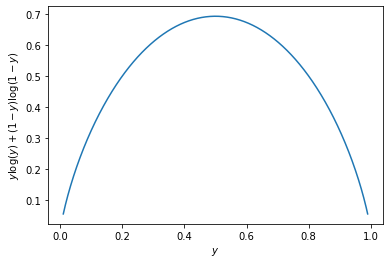
\includegraphics[scale=0.60]{entropy.png}
\end{center}
\caption{The Binary Entropy Function}
\label{fig:binary_entropy}
\end{figure}

\begin{exercise}
Partial derivatives of the cross-entropy cost function in multi-layer
networks.
\end{exercise}
\begin{solution}
The cross-entropy function for a single training example~$x$ for the last
layer~$L$ of the network is defined as:
\[
    C(x) = - \sum_j \left [ y_j \ln (a_j^L) + (1 - y_j) \ln(1 - a_j^L) \right ],
\]
where the sum is over all neurons~$j$ in layer~$L$. To recap notation,  
\[
a_j^L = \sigma(z_j^L) = \sum_k w_{j k}^L a_k^{L - 1} + b_j^L.
\]
For this training example~$x$,
\begin{align*}
    \frac{\partial C(x)}{\partial z_j^L} 
        & = - \frac{y_j}{a_j^L} \cdot \sigma' (z_j^L) + \frac{1 - y_j}{1 - a_j^L} \cdot \sigma' (z_j^L) \\
        & = \frac{-y_j + y_j a_j^L + a_j^L - y_j a_j^L}{a_j^L (1 - a_j^L)} \cdot \sigma' (z_j^L) \\
        & = a_j^L - y_j.
\end{align*}
The last equality follows since $\sigma' (z_j^L) = a_j^L (1 - a_j^L)$.

Again, for this single training example~$x$, $\partial C (x) / \partial w_{j k}^L$ 
is given by:
\begin{align*}
    \frac{\partial C (x)}{\partial w_{j k}^L} 
        & = \frac{\partial C}{\partial z_j^L} \cdot \frac{\partial z_j^L}{\partial w_{j k}^L} \\
        & = (a_j^L - y_j) \cdot a_k^{L - 1}. 
\end{align*}
For $n$ training examples, the cost function is defined as $\frac{1}{n} \sum_{x} C(x)$ and 
this derivative is: 
\[
    \frac{\partial C}{\partial w_{j k}^L} = \frac{1}{n} \sum_x a_k^{L - 1} (a_j^L - y_j).
\]
If we were to replace $C(x)$ by the usual quadratic cost $\frac{1}{2}(y_j - a_j^L)^2$, then 
the same derivative would have been:
\[
    \frac{1}{n} \sum_x a_k^{L - 1} (a_j^L - y_j) \cdot \sigma' (z_j^L).
\]
\end{solution}

\subsection{Deriving the Cross-Entropy Function}

Given a single neuron with $r$ input weights $w_1, \ldots, w_r$ and bias~$b$,
and a single input $\vect{x} = \trans{(x_1, \ldots, x_r)}$, we would like the
cost function $C$ to depend on the weights and the bias as follows:
\begin{align}
    \frac{\partial C}{\partial w_j} & = x_j (a - y) \\
    \frac{\partial C}{\partial b}   & = a - y, \label{eqn:cost_bias}
\end{align}
where $a = \sigma(\sum_{j} w_j x_j + b)$ and $y$ is the desired output 
corresponding to $\vect{x}$. 

Using the chain rule, we obtain:
\begin{align}
    \frac{\partial C}{\partial b} & = 
        \frac{\partial C}{\partial a} \cdot 
        \frac{\partial a}{\partial z} \cdot 
        \frac{\partial z}{\partial b} \nonumber \\
        & = \frac{\partial C}{\partial a} \cdot \sigma'(z) \nonumber \\ 
        & = \frac{\partial C}{\partial a} \cdot a (1 - a) \label{eqn:cross_entropy} 
\end{align}
From equations~(\ref{eqn:cost_bias} and~\ref{eqn:cross_entropy}), we obtain:
\[
    \frac{\partial C}{\partial a} = \frac{a - y}{a (1 - a)} = 
        \frac{1}{1 - a} - y \left ( \frac{1}{1 - a} + \frac{1}{a}\right ).
\]
Integrating both sides wrt~$a$, we obtain:
\[
    C = - [(1 - y) \ln (1 - a) + y \ln (a)] + \text{ a constant}.
\]

\section{Softmax}

Consider a classification problem, where labelled examples take the form 
$(\vect{x}, \vect{y})$, where $\vect{x} \in \R^m$ and $\vect{y} \in \{0, 1\}^J$ 
denotes to which of the $J$ classes $\vect{x}$ belongs to. 
In such cases, it makes sense to have the last 
layer of the neural network to have $J$ neurons with the softmax activation:
\begin{align*}
    z_j^L & = \sum_k w_{j k}^L a_{k}^{L - 1} + b_j \\
    a_j^L & = \frac{e^{z_j^L}}{ \sum_{i = 1}^J e^{z_i^L}}
\end{align*}

The cost associated with the input $(\vect{x}, \vect{y})$ where $y_r = 1$ 
is defined as the negative log-likelihood of the activation $a_{r}^L$:
\[
    C(\vect{x}, \vect{y}) = - \ln a_{r}^L.
\]

The partial derivatives $\partial C / \partial b_j^L$ and   $\partial C / \partial w_{j k}^L$
can be computed easily as follows. Depending on whether the index $j$ and the class index~$r$
are the same or not, we have two cases for each partial derivative.
\begin{align}
    \frac{\partial C}{\partial b_{r}^L} 
        & =   - \frac{1}{a_{r}^L} \cdot 
            \left [ \frac{e^{z_{r}^L}}{ \sum_{i = 1}^J e^{z_i^L}} - 
                    \left ( \frac{e^{z_{r}^L}}{ \sum_{i = 1}^J e^{z_i^L}} \right )^2 
            \right ] = - 1 + a_{r}^L \\
\frac{\partial C}{\partial b_j^L} 
      & = 
    - \frac{1}{a_{r}^L} \cdot \left [ 0 - \frac{e^{z_{r}^L} e^{z_j^L}}{ \left ( \sum_{i = 1}^J e^{z_i^L} \right )^2} 
                            \right ] = a_j^L. 
\end{align}
The first equation is when the index $r = j$ and the second when $r \neq j$. 
These two expressions can be summarized into one: 
\begin{equation}
\frac{\partial C}{\partial b_j^L} = a_{j}^L - y_j.
\end{equation}

Similarly, the partial derivative expression for  $\partial C / \partial w_{j k}^L$
can be written as:
\begin{equation}
\frac{\partial C}{\partial w_{j k}^L} = a_{k}^{L - 1} \cdot (a_{j}^L - y_j). 
\end{equation}

\begin{exercise}
Where does the ``softmax'' name come from? Consider the following variant 
of the softmax function:
\[
    a_j^L =  \frac{e^{c z_j^L}}{ \sum_{i = 1}^J e^{c z_i^L}},
\]
where $c$ is a positive constant. What is the limit of $a_j^L$ 
as $c \to \infty$?
\end{exercise}
\begin{solution}
Let $z_r^L = \max_i \{z_i^L\}$. We could then write the modified softmax
function as:
\[
    a_j^L =  \frac{e^{c (z_j^L - z_r^L)}}{ 1 + \sum_{i \neq r} e^{c (z_i^L - z_r^L)}}. 
\]
If $j = r$, then the numerator is $1$ and the denominator approaches $1$ as $c \to \infty$
and $a_j^L \to 1$. On the other hand, if $j \neq r$, the numerator $\to 0$ as $c \to \infty$;
the denominator in any case approaches~$1$ and hence~$a_j^L \to 0$. The point here is 
that $a_j^L = 1$ if $z_j^L$ is the maximum and $a_j^L = 0$ otherwise. 
\end{solution}

